\documentclass[sigconf]{acmart}

\usepackage{booktabs} % For formal tables
\usepackage{minted}
\usepackage{graphicx}
\usepackage{tabularx}
\usepackage{arydshln}
\usepackage{subcaption}
\usepackage{times}
\usepackage{hyperref}
\usepackage{array}
\usepackage[normalem]{ulem}
\hypersetup{
    colorlinks=true,
    linkcolor=blue,
    filecolor=magenta,      
    urlcolor=cyan,
}
%\setlength{\belowcaptionskip}{-5pt}



% Copyright
\setcopyright{none}
%\setcopyright{acmcopyright}
%\setcopyright{acmlicensed}
%\setcopyright{rightsretained}
%\setcopyright{usgov}
%\setcopyright{usgovmixed}
%\setcopyright{cagov}
%\setcopyright{cagovmixed}


%% DOI
%\acmDOI{10.475/123_4}
%
%% ISBN
%\acmISBN{123-4567-24-567/08/06}
%
%%Conference
%\acmConference[WOODSTOCK'97]{ACM Woodstock conference}{July 1997}{El
%  Paso, Texas USA}
%\acmYear{1997}
%\copyrightyear{2016}
%
%
%\acmArticle{4}
%\acmPrice{15.00}
%
%% These commands are optional
%%\acmBooktitle{Transactions of the ACM Woodstock conference}
%\editor{Jennifer B. Sartor}
%\editor{Theo D'Hondt}
%\editor{Wolfgang De Meuter}


\begin{document}
\title{Popper Pitfalls: Experiences Following the Popper Convention}

\author{Michael A. Sevilla}
\affiliation{%
 \institution{University of California, Santa Cruz}}
\email{msevilla@soe.ucsc.edu}

\author{Carlos Maltzahn}
\affiliation{%
  \institution{University of California, Santa Cruz}}
\email{carlosm@ucsc.edu}

\begin{abstract}

We describe the four publications we have tried to make reproducible and
discuss how each paper has changed our workflows, practices, and collaboration
policies. The fundamental insight is that paper artifacts must be made
reproducible from the start of the project; artifacts are too difficult to make
reproducible when the papers are (1) already published and (2) authored by
researchers that are not thinking about reproducibility. In this paper, we
present the best practices adopted by our research laboratory, which was
sculpted by the pitfalls we have identified for the Popper convention.  We
conclude with a ``call-to-arms" for the community focused on enhancing
reproducibility initiatives for academic conferences, industry environments,
and national laboratories. We hope that our experiences will shape a best
practices guide for future reproducible papers.

\end{abstract}



%
% The code below should be generated by the tool at
% http://dl.acm.org/ccs.cfm
% Please copy and paste the code instead of the example below.
%
%\begin{CCSXML}
%<ccs2012>
% <concept>
%  <concept_id>10010520.10010553.10010562</concept_id>
%  <concept_desc>Computer systems organization~Embedded systems</concept_desc>
%  <concept_significance>500</concept_significance>
% </concept>
% <concept>
%  <concept_id>10010520.10010575.10010755</concept_id>
%  <concept_desc>Computer systems organization~Redundancy</concept_desc>
%  <concept_significance>300</concept_significance>
% </concept>
% <concept>
%  <concept_id>10010520.10010553.10010554</concept_id>
%  <concept_desc>Computer systems organization~Robotics</concept_desc>
%  <concept_significance>100</concept_significance>
% </concept>
% <concept>
%  <concept_id>10003033.10003083.10003095</concept_id>
%  <concept_desc>Networks~Network reliability</concept_desc>
%  <concept_significance>100</concept_significance>
% </concept>
%</ccs2012>
%\end{CCSXML}

%\ccsdesc[500]{Computer systems organization~Embedded systems}
%\ccsdesc[300]{Computer systems organization~Redundancy}
%\ccsdesc{Computer systems organization~Robotics}
%\ccsdesc[100]{Networks~Network reliability}


%\keywords{ACM proceedings, \LaTeX, text tagging}

\maketitle

\section{Introduction}

\section{Popper-compliant Papers}

% what papers have we done
We have authored five Popper-compliant papers:
\begin{itemize}

\item quiho: Automated Performance Regression Testing Using Inferred
Resource Utilization Profiles

\item Cudele: An API and Framework for Programmable Consistency and
Durability in a Global Namespace

\item Malacology: A Programmable Storage System

\item Characterizing and Reducing Cross-Platform Performance Using
OS-level Virtualization

\item Programmable Caches with a Data Management Language \& Policy Engine

\end{itemize}

Popper 


\section{Reproducibility Must Be a 1st Class Citizen}
% exploration vs. complete
% cross-cluster compatibility 
%  - inventory files hard coded throughout tree
%  - configuration files not propagated for experiments
%  - visualize files pulled data from hard coded paths
%  - graphs not created automatically
% why Mantle failed

\section{Organized Repositories and Documentation}
%cause the most work
% role of git
% docker images saved in internal registry (buildding)

\section{Well-Defined Collaboration Roles}
% keeping organization
% workflows

\section{Maintaining Pointers}
% wary of ephemeral links

% large code bases large code bases (src, deploy)

% different registry hubs (Docker, GitHub)

\section{Conference Requirements}
% double blinded??

\section{Conclusion}

\section{Popper-compliant Papers}
\label{sec:popper-compliant-papers}

We have produced four Popper-compliant papers, as shown in
Table~\ref{table:papers}. These papers follow the reader/reviewer sample
workflow outlined in~\cite{jimenez:ipdpsw17-popper} and shown in
Figure~\ref{fig:workflow}. For the visualization component (1), we use Jupyter
notebooks. The notebooks themselves are versioned with Git and users interact
with local copies by cloning the repository and launching a Jupyter Docker
container. The paper is written in \LaTeX and built with a Docker container.
For the code component (2), both the source code for the system itself and the
deploy/experiment code is stored on GitHub. When running experiments, we use
Docker containers to isolate libraries and binaries. For the multi-node
component (3), we use CloudLab machines and Ansible to script deployment and
experiment orchestration. For the data set components (4), we use GitHub to
store results files; our inputs and results are small enough that we do no need
a larger capacity.  GitHub allows files up to 50MB and stores data on S3.

Our experiments start with a baseline. To describe the process, we reference
our
ceph-popper-template\footnote{https://github.com/michaelsevilla/ceph-popper-template}
set up on CloudLab. Users setup SSH keys and deploy CloudLab nodes using our
CephFS Profile\footnote{https://www.cloudlab.us/p/CephFS/CephFS-HEP}.  The
profile has the nodes automatically install Docker on bootup using our
install\footnote{https://github.com/michaelsevilla/ceph-popper-template/blob/master/hardware/cloudlab/\-install.sh}
script. After the nodes finish booting ({\it i.e.}  their status on the
CloudLab GUI is READY), users push SSH keys using a convenience
script\footnote{https://raw.githubusercontent.com/michaelsevilla/ceph-popper-template/master/hardware/cloudlab/pushkeys.sh}.

The deploy code is based on
ceph-ansible\footnote{https://github.com/ceph/ceph-ansible/wiki}, a tool that
configures hardware and software for Ceph. We forked the project and made it
less dependent on Python. To run an experiment, users log into the head node
and clone the ceph-popper-template repository. This repository has submodules
that point to ceph-ansible and our own custom roles; configuration files for
our Ceph setup; and helper scripts written in bash that deploy Ceph and run the
benchmarks.  For more information on the Ceph template, see the
README\footnote{https://github.com/michaelsevilla/ceph-popper-template} and for
more information on the baseline and pipelines terminology, see the Popper
Convention quickstart\footnote{http://falsifiable.us/}. 

\begin{figure}[tb] 
  \centering
  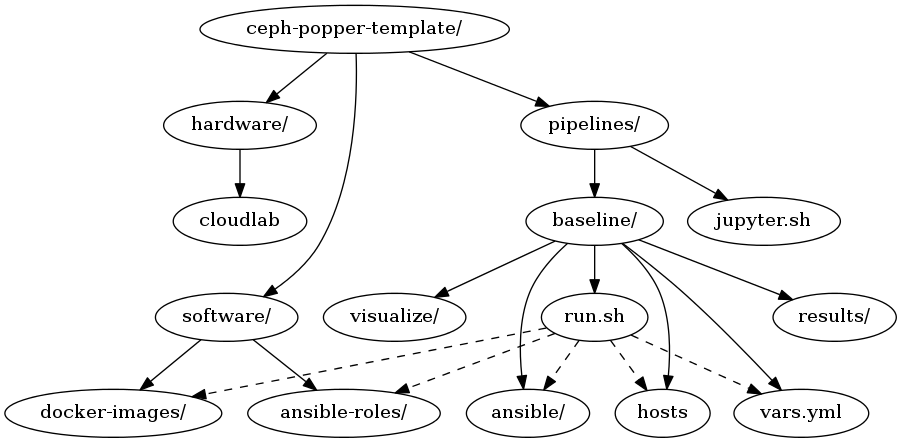
\includegraphics[width=1\linewidth]{./figures/expdir.png}
  \caption{Organization of our experiment directories. \texttt{baseline/} is an
example experiment and contains scripts populated with the Popper CLI. The
\texttt{run.sh} script uses many directories and files to setup and run
experiments, as indicated by the dashed lines.}
  \label{fig:expdir}
\end{figure}

An outline of this organization is shown in Figure~\ref{fig:expdir}, where
solid lines are directory links and dashed lines indicate which directories a
script uses.  A sample experiment is in the \texttt{baseline/} directoriy,
which was created using the Popper CLI. Users configure their cluster by
specifying hostnames and login user names in the \texttt{hosts} file.  Users
also specify the Ceph services that should be deployed using the
\texttt{ansible/}
directory\footnote{https://github.com/michaelsevilla/ceph-popper-template/tree/master/pipelines/baseline/ansible}.
This directory has code for deploying Ceph and its components, where the
\texttt{*.yml} files are Ansible playbooks that start and configure components:
\texttt{ceph.yml} starts Ceph and can be modified to specify which daemons to
launch, \texttt{cleanup.yml} tears Ceph down, and \texttt{monitor.yml} starts
daemons that monitor performance.  High level configurations are in the
\texttt{vars.yml} file.  We separate these components into different playbooks
so users can mix and match Ceph services.  Similarly, the workloads directory
has scripts for running the baseline benchmarks. The other files and
directories are Ansible configuration files used by the playbooks. We have
posted a tutorial on our
blog\footnote{http://programmability.us/mantle/blog2-ceph} to guide users
through this setup. When complete, users execute the \texttt{run.sh} to start
the job.



\section{Conclusion}

We have outlined the structure of our ``reproducible" papers and showed the
complexity of researching in this way. We iterated to a Popper-compliant
paper-writing process after encountering numerous pitfalls, which we have
documented and used to shape our best practices. While our process will never
be perfect, we are encouraged with the improved speed and ease that our research
progresses now that we have: (1) made reproducibility a 1st class citizen, (2)
defined collaboration rules, and (3) made it a priority to maintain pointers.
We hope that our call-to-arms for community cooperation effectively improves
the state of reproducibility in the field.

Our future work is to quantify the efficiency improvements or degradations in
efficiency due to reproducibility. An effective way to quantify productivity,
in addition to the time spent on a problem, would help us more concretely
identify when the reproducibility approach is useful or not. It might also help
us explore other environments where reproducibility is useful, such as the
classroom or in conference settings. Finally, it would highlight situations
where the extra time spent setting up workflows and building paper artifacts is
{\it worth it} for the ultimate payout of reproducibility when the paper is
published.


\bibliographystyle{ACM-Reference-Format}
\bibliography{paper}
\end{document}

